% !TEX TS-program = XeLaTeX
% use the following command:
% all document files must be coded in UTF-8
\documentclass[english]{textolivre}
% build HTML with: make4ht -e build.lua -c textolivre.cfg -x -u article "fn-in,svg,pic-align"

\journalname{Texto Livre}
\thevolume{18}
%\thenumber{1} % old template
\theyear{2025}
\receiveddate{\DTMdisplaydate{2024}{12}{19}{-1}} % YYYY MM DD
\accepteddate{\DTMdisplaydate{2025}{2}{26}{-1}}
\publisheddate{\DTMdisplaydate{2025}{6}{7}{-1}}
\corrauthor{William Gottardi}
\articledoi{10.1590/1983-3652.2025.56636}
%\articleid{NNNN} % if the article ID is not the last 5 numbers of its DOI, provide it using \articleid{} commmand 
% list of available sesscions in the journal: articles, dossier, reports, essays, reviews, interviews, editorial
\articlesessionname{dossier}
\runningauthor{Gottardi and Silveira} 
%\editorname{Leonardo Araújo} % old template
\sectioneditorname{Hugo Heredia Ponce}
\layouteditorname{Leonado Araújo}

\title{A theoretical assessment of ASR-based pronunciation activities for classroom learning}
\othertitle{Avaliação teórica de atividades de pronúncia baseadas em tecnologia de reconhecimento de fala para aprendizagem em sala de aula}
% if there is a third language title, add here:
%\othertitle{Artikelvorlage zur Einreichung beim Texto Livre Journal}

\author[1]{William Gottardi~\orcid{0000-0002-1291-3953}\thanks{Email: \href{mailto:prof.williamgottardi@outlook.com}{prof.williamgottardi@outlook.com}}}
\author[1]{Rosane Silveira~\orcid{0000-0003-0329-0376}\thanks{Email: \href{mailto:rosanesilduarte@gmail.com}{rosanesilduarte@gmail.com}}}
\affil[1]{Federal University of Santa Catarina, English: Linguistic and Literary Studies Program, Department of Foreign Languages and Literature, Florianópolis, SC, Brazil.}

\addbibresource{article.bib}
% use biber instead of bibtex
% $ biber article

% used to create dummy text for the template file
\definecolor{dark-gray}{gray}{0.35} % color used to display dummy texts
\usepackage{lipsum}
\SetLipsumParListSurrounders{\colorlet{oldcolor}{.}\color{dark-gray}}{\color{oldcolor}}

% used here only to provide the XeLaTeX and BibTeX logos
\usepackage{hologo}

% if you use multirows in a table, include the multirow package
\usepackage{multirow}

% provides sidewaysfigure environment
\usepackage{rotating}

% CUSTOM EPIGRAPH - BEGIN 
%%% https://tex.stackexchange.com/questions/193178/specific-epigraph-style
\usepackage{epigraph}
\renewcommand\textflush{flushright}
\makeatletter
\newlength\epitextskip
\pretocmd{\@epitext}{\em}{}{}
\apptocmd{\@epitext}{\em}{}{}
\patchcmd{\epigraph}{\@epitext{#1}\\}{\@epitext{#1}\\[\epitextskip]}{}{}
\makeatother
\setlength\epigraphrule{0pt}
\setlength\epitextskip{0.5ex}
\setlength\epigraphwidth{.7\textwidth}
% CUSTOM EPIGRAPH - END

% to use IPA symbols in unicode add
%\usepackage{fontspec}
%\newfontfamily\ipafont{CMU Serif}
%\newcommand{\ipa}[1]{{\ipafont #1}}
% and in the text you may use the \ipa{...} command passing the symbols in unicode

% LANGUAGE - BEGIN
% ARABIC
% for languages that use special fonts, you must provide the typeface that will be used
% \setotherlanguage{arabic}
% \newfontfamily\arabicfont[Script=Arabic]{Amiri}
% \newfontfamily\arabicfontsf[Script=Arabic]{Amiri}
% \newfontfamily\arabicfonttt[Script=Arabic]{Amiri}
%
% in the article, to add arabic text use: \textlang{arabic}{ ... }
%
% RUSSIAN
% for russian text we also need to define fonts with support for Cyrillic script
% \usepackage{fontspec}
% \setotherlanguage{russian}
% \newfontfamily\cyrillicfont{Times New Roman}
% \newfontfamily\cyrillicfontsf{Times New Roman}[Script=Cyrillic]
% \newfontfamily\cyrillicfonttt{Times New Roman}[Script=Cyrillic]
%
% in the text use \begin{russian} ... \end{russian}
% LANGUAGE - END

% EMOJIS - BEGIN
% to use emoticons in your manuscript
% https://stackoverflow.com/questions/190145/how-to-insert-emoticons-in-latex/57076064
% using font Symbola, which has full support
% the font may be downloaded at:
% https://dn-works.com/ufas/
% add to preamble:
% \newfontfamily\Symbola{Symbola}
% in the text use:
% {\Symbola }
% EMOJIS - END

% LABEL REFERENCE TO DESCRIPTIVE LIST - BEGIN
% reference itens in a descriptive list using their labels instead of numbers
% insert the code below in the preambule:
%\makeatletter
%\let\orgdescriptionlabel\descriptionlabel
%\renewcommand*{\descriptionlabel}[1]{%
%  \let\orglabel\label
%  \let\label\@gobble
%  \phantomsection
%  \edef\@currentlabel{#1\unskip}%
%  \let\label\orglabel
%  \orgdescriptionlabel{#1}%
%}
%\makeatother
%
% in your document, use as illustraded here:
%\begin{description}
%  \item[first\label{itm1}] this is only an example;
%  % ...  add more items
%\end{description}
% LABEL REFERENCE TO DESCRIPTIVE LIST - END


% add line numbers for submission
%\usepackage{lineno}
%\linenumbers

\usepackage{tipa}

\begin{document}
\maketitle

\begin{polyabstract}
\begin{abstract}
The use of digital technologies in the daily routine
of second language (L2) classes became unavoidable when teachers needed
to overcome mobility restrictions imposed by the COVID-19 pandemic. In
countries where access to technological resources in regular classrooms
is still limited, the use of free digital resources for pedagogical
purposes is a valuable alternative. This pedagogical paper explores the
use of Automatic Speech Recognition (ASR) for L2 pronunciation teaching
and learning. Three ASR-based activities drawn from \textcite{gottardi2023} are
presented and discussed. The assessment is based on the criteria
provided by two frameworks. From the pedagogical perspective, we adopted
the communicative pronunciation teaching framework \cite{celcemurcia2010}, which proposes five steps to teach pronunciation
and design materials, including explicit instruction, perception, and
production tasks, with different degrees of teacher guidance and
feedback. Considering the use of technology and the design of
pedagogical activities, we draw on \posscite{chapelle2001} six criteria to
evaluate educational software and activities. We analyzed each ASR-based
pronunciation activity in terms of language learning potential, learner
fit, meaning focus, authenticity, positive impact, and practicality.
Thus, the objective of this pedagogical paper is to 1) discuss how ASR
technology can assist L2 pronunciation practice; 2) provide practical
examples of ASR-based pronunciation activities designed to be used by L2
teachers; and 3) examine the pedagogical appropriateness of the proposed
activities. Finally, pedagogical implications of using ASR for
pronunciation practice are discussed.

\keywords{Computer-Assisted Language Learning \sep Pronunciation
teaching \sep Pronunciation learning \sep Automatic Speech Recognition \sep
Intelligibility}
\end{abstract}

\begin{portuguese}
\begin{abstract}
O uso de tecnologias digitais em aulas de uma
segunda língua (L2) tornou-se inevitável quando os professores
precisaram enfrentar as restrições de mobilidade impostas pela pandemia
do COVID-19. Nos países onde o acesso a recursos tecnológicos nas salas
de aula ainda é limitado, a utilização de recursos digitais gratuitos
para fins pedagógicos é uma alternativa valiosa. Este artigo apresenta
uma reflexão sobre o uso de Reconhecimento Automático da Fala (ASR --
\emph{Automatic Speech Recognition}) aplicado no ensino e aprendizagem
da pronúncia de L2. Três atividades que utilizam a tecnologia de ASR
\cite{gottardi2023} são apresentadas e discutidas. A avaliação se apoia
em critérios fornecidos por dois modelos teóricos. Foi adotado o
referencial de ensino comunicativo da pronúncia \cite{celcemurcia2010},
o qual inclui cinco etapas para o ensino de pronúncia e elaboração de
materiais, contendo momentos de instrução explícita e tarefas de
percepção e produção, com diferentes graus de feedback e mediação do
professor. Recorremos aos critérios de \textcite{chapelle2001} para avaliar
atividades e \emph{softwares} educacionais, o qual nos permitiu analisar
as atividades de pronúncia em termos de: potencial de aprendizagem da
língua, adequação ao aprendiz, foco no significado, autenticidade,
impacto positivo e praticidade. Assim, os objetivos deste artigo
pedagógico são: 1) discutir como a tecnologia de ASR pode auxiliar na
prática da pronúncia de uma segunda língua; 2) fornecer exemplos
práticos de atividades de pronúncia que fazem uso de ASR, mediadas por
professores de L2; e 3) examinar a adequação pedagógica das atividades
propostas. Por fim, implicações pedagógicas são discutidas em relação ao
uso de ASR para a prática de pronúncia.

\keywords{Aprendizagem de Línguas Mediada por Computador \sep
Ensino da pronúncia \sep Aprendizagem de pronúncia \sep Reconhecimento
Automático da Fala \sep Inteligibilidade}
\end{abstract}
\end{portuguese}
% if there is another abstract, insert it here using the same scheme
\end{polyabstract}

\section{Introduction}\label{sec-intro}

The term pronunciation encompasses ``all aspects of how we employ speech
sounds for communicating'' \cite[p.~247]{burns2020} not being
limited to single sounds since it comprehends other speech features such
as segments, prosody, and connected speech phenomena \cite{cardoso2017}.
Although pronunciation can be seen as an essential element of successful
spoken communication \cite{baldissera2021,pennington2019}, it ``has
been historically under-represented and overlooked in comparison to
other areas of second language acquisition research'' \cite[p.~75]{foote2017}.


Furthermore, pronunciation teaching is commonly neglected in second
language\textsuperscript{\footnote{The term second language will be used
  throughout the article with no distinction between English as a
  foreign, second, lingua franca, or additional language (see \textcite{jordao2014} for a meticulous definition of these terms).}} (L2) classrooms,
which is not surprising since the field of second language acquisition
(SLA) has historically marginalized pronunciation from both theoretical
and pedagogical perspectives \cite{olson2023}. Also, time dedicated to
the teaching of L2 pronunciation is limited by an overloaded syllabus
\cite{collins2016}.


Bearing this scenario in mind, the use of digital technology --
particularly speech technologies -- can help mitigate this time
constraint \cite{gottardi2022,silveira2022}. For example, Automatic
Speech Recognition (ASR) is a speech technology with proven positive
impact on L2 learning that can foster learners' autonomy by engaging
them in extended pronunciation practice \cite{gottardi2022}. In short, the
use of ASR technology might be an alternative to circumvent time
constraints related to an overloaded curriculum and provide learners
with more pronunciation practice opportunities.

Considering the new scenario brought about by the COVID-19 pandemic that
``pushed virtually all teachers to teach via technological mediation''
\cite[p.~529]{kern2024}, investigation into new digital technologies to
assist language teaching and learning is welcome, especially the ones
that can be applied into different teaching contexts as well as
autonomous learning, as is the case with ASR technology. Thus,
pedagogical reflections on the use of ASR as a teaching resource and
suggestions on how to integrate it into teachers' practices are relevant
if the guiding role played by the teacher is taken into account as well
as their needs for support and assistance.


All in all, this pedagogical paper has the aim of 1) discussing how ASR
technology can aid L2 pronunciation practice; 2) providing practical
suggestions of ASR-based pronunciation activities designed to be used by
L2 teachers; and 3) examining the appropriateness of these pronunciation
activities from a pedagogical perspective.

In the following sections, we review relevant literature concerning L2
pronunciation teaching dimensions, priorities and a framework for
designing pronunciation teaching materials. Then, we discuss important
issues related to digital technologies and L2 pronunciation teaching.
Section 4 brings a discussion about ASR for L2 pedagogical purposes
followed by the analysis of three pronunciation activities designed to
be implemented in L2 classes mediated by teachers.


\section{Pronunciation teaching}\label{pronunciation-teaching}

Pronunciation is an essential component
targeting successful spoken communication \cite{pennington2019} and
is closely linked to social issues since it ``cannot be ignored in view
of globalization, the growing needs of cross-cultural communication, and
issues of speaker identity and social integration'' \cite[p.~213]{chun2020}.

In the field of L2 pronunciation, speech is often divided into three
different dimensions, namely: \emph{intelligibility},
\emph{comprehensibility}, and \emph{accentedness}. Following \textcite[p.~5]{derwing2015}, intelligibility can be defined as ``the degree of
match between the speaker's intended message and listener's
comprehension''. Furthermore, the authors define comprehensibility as
the degree of difficulty in understanding speech based on the listener's
estimation. Lastly, accentedness refers to how different the speech is
from the expected production patterns of a speech community.

Current views of L2 pronunciation teaching, based on the findings of L2
speech research, advocate a focus on enhancing intelligibility and
comprehensibility, considering that accent is ubiquitous and striving
for native-like pronunciation is considered an inadequate goal
\cite{obrien2018}. Likewise, \textcite{levis2020} contends that focusing
pronunciation teaching on intelligibility aligns with realistic goals
since accent should be seen as a variation to embrace instead of a
problem to overcome.


In addition, communication is the primary purpose of language use.
Hence, the main goal of L2 teaching should be using language to
communicate \cite{celcemurcia2010}. Following this principle, \textcite{celcemurcia2010} proposed a framework for pronunciation teaching based on
the tenets of communicative language teaching (CLT). \Cref{tbl01} summarizes
this framework, which considers the learners' gradual development of new
L2 pronunciation features.


\begin{table}[htpb]
\centering
\begin{threeparttable}
\caption{Communicative framework for teaching English pronunciation.}
\label{tbl01}
\begin{tabular}{lp{10cm}}
\toprule
1- Description and analysis & Oral and written illustrations of how the
feature is produced and when it occurs within spoken discourse. \\
2- Listening discrimination & Focused listening practice with feedback
on learners\textquotesingle{} ability to correctly discriminate the
feature. \\
3- Controlled practice & Oral reading of minimal-pair sentences, short
dialogues, etc., with special attention paid to the highlighted feature
in order to raise learner\textquotesingle s consciousness. \\
4- Guided practice & Structured communication exercises, such as
information-gap activities or cued dialogues, that enable the learner to
monitor for the specified feature. \\
5- Communicative practice & Less structured, fluency-building activities
(e.g., role play, problem solving) that require the learner to attend to
both form and content of utterances. \\
\bottomrule
\end{tabular}
\source{\textcite[p.~45]{celcemurcia2010}}
\end{threeparttable}
\end{table}



The above-mentioned framework suggests a 5-phase division of the
pronunciation lesson. The first phase focuses on phonological awareness,
the second focuses on perception skills while the last three phases
address the learner's production. The framework recognizes that
pronunciation learning is not a linear process. Therefore, teachers
might need to revisit certain phases during their teaching process. The
authors of this framework also advocate setting realistic goals for
pronunciation teaching, ``focusing on the targeted communicative needs
of {[}\ldots{]} learners, not the language as a whole'' \cite[p.~283]{celcemurcia2010}.

Considering the arguments presented in this section, pronunciation
teaching and learning are of pivotal importance when it comes to
achieving intelligible speech, aiming at successful communication. As
\textcite[p.~219]{pennington2019} contend, ``having a
critical awareness of pedagogic resources and related research can help
teachers make informed choices about what and how to teach''. In
addition, pronunciation learning is highly affected by learners'
exposure to the L2 as well as the extent to which they actually use it
\cite{lane2010}. Therefore, digital resources may help learners to have
more L2 exposure as well as teachers to achieve their pedagogical goals.
The next section discusses the relationship between digital technologies
and pronunciation teaching.


\section{Contributions of digital technologies to pronunciation
teaching}\label{sec-contributions}

Digital technologies grant access for people to ``speak or write either
synchronously or asynchronously, with participants either at a distance
or in close proximity'' \cite[p.~66]{chun2016}. Nevertheless, the use
of digital technology should not be considered the solution to all
problems, but rather a way of supporting specific pedagogical goals
\cite{chun2016}, such as offering varied oral input and immediate
feedback to learners \cite{baldissera2021}.


Moreover, digital technologies may allow learners to be more autonomous
toward their learning process, besides promoting learning beyond the
classroom \cite{lai2018}. In a similar vein, \textcite[p.~336]{thomson2015} contend that ``computer-based approaches may promote greater
learner autonomy and, most importantly, afford the possibility of
individualized instruction''. Finally, technology can also offer ``the
learner limitless choice of what, when, and how to learn''
\cite[p.~201]{rogersonrevell2021}.

This complex nature of technology and pedagogy demanded the creation of
a new subfield of applied linguistics called Computer-Assisted Language
Learning (CALL), which studies the relationship between technology and
L2 learning \cite{martins2012}. Simply put, CALL is ``an approach to
language teaching and learning in which computer technology is used as
an aid to the presentation, reinforcement, and assessment of material to
be learned'' \cite[p.~261]{davies2006}.

In recent decades, this field has advanced quickly
\cite{pennington2019} and new digital resources are made available
to teachers and learners all the time. Although having access to more
CALL resources might be a positive asset, it can also represent an extra
challenge for both educators and students to stay updated with the
latest releases \cite{soleimani2021}. Thus, evaluating CALL software and
the activities designed to use CALL resources is relevant since it is
what ``teachers need to concentrate more on, in order to ensure that
technology is not used for technology\textquotesingle s sake'' \cite[p.~9]{stanley2013}.

The evaluation of CALL learning activities can be challenging. However,
it is necessary in order to assess how pedagogically adequate the
digital resources are and how appropriate the CALL activity is to
learners' needs. According to \textcite{chapelle2017}, a possible way of
evaluating the appropriateness of L2 teaching materials and positive
aspects of learning activities is by making a pedagogy‐based argument.
Following this line of argumentation, \textcite{chapelle2001} suggests a set of
SLA-grounded criteria (see \Cref{tbl02} below) that can be applied to
evaluating educational software and activities that teachers plan to use
in their classes. Adopting such a framework can help ``support claims
about the value of technology‐mediated learning for meeting pedagogical
requirements'' \cite[p.~386]{chapelle2017}.


\begin{table}[htpb]
\centering
\begin{threeparttable}
\caption{The six criteria for assessing CALL task appropriateness.}
\label{tbl02}
\begin{tabular}{lp{11cm}}
\toprule
\multicolumn{1}{p{3cm}}{1- Language learning potential} & The degree of opportunity present for
beneficial focus on form. \\
2- Learner fit & The amount of opportunity for engagement with language
under appropriate conditions given learner characteristics. \\
3- Meaning focus & The extent to which learners' attention is directed
toward the meaning of the language. \\
4- Authenticity & The degree of correspondence between the CALL activity
and target language activities of interest to learners out of the
classroom. \\
5- Positive impact & The positive effects of the CALL activity on those
who participate in it. \\
6- Practicality & The adequacy of resources to support the use of the
CALL Activity. \\
\bottomrule
\end{tabular}
\source{\textcite[p.~55]{chapelle2001}}
\end{threeparttable}
\end{table}




The language learning potential criterion evaluates whether the activity
is a proper language learning activity instead of a simple opportunity
for language use, that is, the activity can promote a beneficial focus
on linguistic forms. Although the importance of each criterion may
differ according to the objective of the task, language learning
potential ``should be considered the most critical for CALL activities''
\cite[p.~58]{chapelle2001}.

The learner fit criterion refers to how appropriate the activity is for
the learner, considering the difficulty level, and the learner's
individual differences and characteristics. The meaning focus criterion
evaluates if the activity directs learners' primary attention to the
meaning of the language required to accomplish the task. This criterion
also takes into account activities that involve using language skills
for the interpretation and construction of meaning.


The authenticity criterion analyses whether the learning task is similar
to a task that learners would expect to see outside of the L2 classroom.
As \textcite[p.~56]{chapelle2001} states, ``the criterion of authenticity
indicates the need to develop learners' willingness to communicate, but
it also extends beyond the conditions believed important for
acquisition''; therefore, activities should offer opportunity to
interact with other language users and to generate more spoken output.

The positive impact criterion evaluates if the learning task teaches
more than language, that is, supports learners to develop or improve
their metacognitive strategies, allowing them to claim agency over their
learning process. It also evaluates if both teachers and learners might
have a positive learning experience during the activity.

Finally, the practicality criterion evaluates whether the learning task
is easy for the teachers and learners to implement considering the
particular constraints of an L2 class or a language program. In
addition, this last criterion takes into account the availability of
software, hardware, and knowledgeable personnel needed for the proper
execution of the learning task \cite{chapelle2001}.


All things considered, the benefits of current digital technologies to
pronunciation teaching are enormous \cite{obrien2018}, and the advances
in computer technology have considerably contributed to the improvement
of L2 teaching and learning \cite{cardoso2022}. Nonetheless, a
particular speech technology, Automatic Speech Recognition (ASR), may be
a suitable CALL resource as ASR-based pronunciation activities have the
potential to fulfill the aforementioned criteria proposed by \textcite{chapelle2001},
as we shall see next.



\subsection{Automatic speech recognition and L2
pronunciation}\label{sec-automatic}


Simply stated, ASR is ``an independent, machine-based process of
decoding and transcribing oral speech'' \cite[p.~149]{levis2020b}; that
is, it transcribes oral input (speech) into orthographic output.
Although ASR technology is not recent, since the first ASR systems date
back to the 1950s, recent years witnessed an accelerated improvement in
its capabilities due to the development of more robust algorithms and
new model techniques, the expanding demand for ASR integration with
smart devices, and the improvement in noisy speech recognition
\cite{jurafsky2024,levis2020b}. Throughout these years, much progress
has been made, allowing the current level of speech recognition accuracy
exceeding 95\% \cite{cardoso2022}.

ASR technology has improved to the extent that it is suitable for many
tasks. It can be embedded into smart devices containing Intelligent
Personal Assistants (IPAs) (e.g., Google Assistant, Siri, Alexa), used
to auto-generate captions, applied to human-computer interaction, or
dictation tools \cite{jurafsky2024,vanlieshout2022}.

In recent years, two significant events have occurred that have
attracted the interest of both the academic community and
tech-companies. First, the impact of Covid-19 on educational contexts
that ``led to educational technology being used for learning out of
school, at a pace and scale with no historical precedent''
\cite[p.~13]{unesco2023}. Second, the emergence of generative Artificial
Intelligence (AI)-powered chatbots, or AI-powered assistants, which
allow users to have conversations with a virtual assistant while
searching and generating content \cite{ibm2024}.

When it comes to the affordances and limitations of ASR for L2 learning
and teaching, especially for pronunciation development, much research
has been conducted in the past decade\textsuperscript{\footnote{For a
  reflection on this topic until the beginning of this decade, see \textcite{gottardi2022}.}}. First, teachers seem to hold a
positive attitude towards ASR for pronunciation teaching
\cite{gottardi2024}. Also, ASR's capacity to generate instant
orthographic feedback may help learners to be more independent in their
learning process and this corrective feedback might be useful for
pronunciation learning \cite{liakina2022}. Finally, ASR tools may help
learners to be more autonomous, working as a valuable self-directed
language learning resource \cite{cardoso2022}.

Furthermore, as stated by \textcite[p.~778]{kivistodesouza2022},
ASR tools ``can be a helpful additional pronunciation learning tool for
L2 users'', especially because they might assist learners in noticing
pronunciation patterns that hinder communication. In a similar vein,
\textcite[p.~14]{santos2024} state that using ASR to
practice isolated words ``may still play a significant role in
contributing with the noticing of specific phonological issues at the
segmental level''. ASR has also been shown to improve learners'
pronunciation and that they tend to have a positive attitude toward ASR
tools \cite{nickolai2024}.

On the other hand, ASR can present pedagogical limitations and potential
biases. ASR accuracy is significantly reduced if input speech contains
distortions, is spoken far from the recording microphone, in a noisy
environment, or the speaker's accent is too different from those used to
train the ASR program; that is, native-accented speech may be more
easily recognized by ASR systems \cite{jurafsky2024,oshaughnessy2024}.

In summary, to consider ASR as a pedagogical resource, it is important
to have an overview of all the recent technological advances and current
limitations. Notwithstanding, ASR affordances for pronunciation teaching
and learning are numerous. Thus, knowing how to implement ASR tools in
an L2 classroom may be a valuable pedagogical skill for teachers. In the
next section, ASR-based pronunciation activities are presented and
analyzed with the help of the two theoretical frameworks described in
sections 2 and 3.



\section{Assessing ASR-based activities designed for pronunciation
teaching}\label{sec-assessing}

In the following sub-sections, three ASR-based pronunciation activities
are presented. The activities were part of a set of seven activities
proposed by \textcite{gottardi2023} and intended for implementation in L2
English classes. We selected three activities to analyze their
appropriateness according to the criteria of the frameworks proposed by \textcite{celcemurcia2010,chapelle2001}.

The activities were designed following the same structure as the
activities by \textcite{stanley2013}; that is, starting with a table which
provides the L2 teacher with a summary of the main pedagogical aspects
of the activity, followed by the procedures to implement the activities,
possible variations and an appendix containing a handout to give to the
students. Each activity aims at a specific Common European Framework of
Reference for Languages (CEFR) proficiency level range. For readability
improvement, only the summary table is displayed during the pedagogical
analyses. The complete version of the activities can be found in the
appendices.


Every activity suggests a specific dictation passage to be used to
interact with the selected ASR tool. The ASR tool employed during the
activities was Google Translate's ASR feature (hereafter, GT). GT is a
highly accessible tool available for free as a website or a mobile app,
particularly popular in Brazil \cite{google2016}. In addition, it is
constantly improving and updating its speech features
\cite{cardoso2022}, which makes GT an adequate source of the latest
improvements in ASR technology.

Considering the technological requirements, all three activities need
the same infrastructure for their implementation: a digital device
(e.g., personal computer, laptop, a smartphone with Google Translate's
app installed), stable internet connection, and an input device (e.g.,
microphone, headphone, cellphone's microphone). \Cref{fig01} below shows
Google Translate's speech features. Before using the web version of GT,
however, it is important to allow the browser to use computer's
microphone. Also, it is necessary to choose the language to translate
to, in this case, English \cite{google2024}.


\begin{figure}[htbp]
\centering
\begin{minipage}{.5\textwidth}
 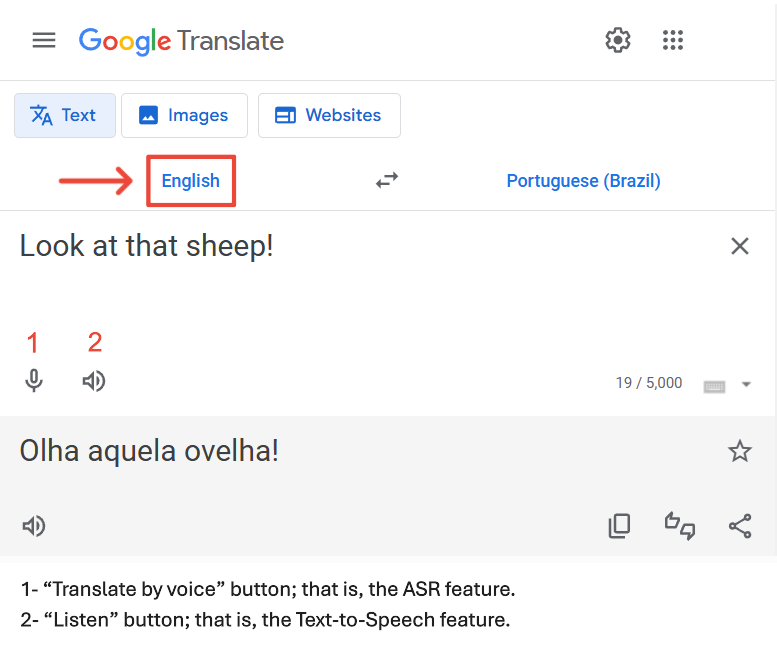
\includegraphics[width=\textwidth]{fig01.png}
 \caption{Google Translate's features on a browser.}
 \label{fig01}
 \source{The authors.}
\end{minipage}
\end{figure}

From a pedagogical viewpoint, each pronunciation activity explores
different teaching techniques for L2 pronunciation practice and
addresses different phases of the Communicative Framework for Teaching
Pronunciation from Celce-Murcia et al.~(2010). Additionally, the
activities address different pronunciation target features, chosen based
on recurring learning difficulties found among L2 Brazilian learners
\cite{zimmer2009} and typical intelligibility issues in their speech
\cite{goncalves2015,silveira2017}. Lastly, the activities were designed
bearing in mind the six Criteria for CALL Task Appropriateness from \cite{chapelle2001}.

In summary, the rationale informing the design of the ASR-based
pronunciation activities was provided. In this research context,
learners' intelligibility issues and pronunciation difficulties were
prioritized when designing the activities. The following sections
present a more detailed pedagogical analysis of the activities.


\subsection{Activity 1 -- pronunciation self-assessment}\label{sec-activity-1}

The Pronunciation Self-Assessment activity (see \Cref{tbl03} and \Cref{apdx1})
brings a classic communicative activity that involves completing a
worksheet containing short sentences for self-introduction. It is an
opportunity for guided pronunciation practice because the worksheet
brings sentence templates that learners are supposed to complete with
personal information. Furthermore, it can be used as an initial step for
learners to feel more confident to prepare to interact with a classmate,
sharing their personal information and getting to know each other.


\begin{table}[htpb]
\centering
\begin{threeparttable}
\caption{Summary of Activity 1.}
\label{tbl03}
\begin{tabular}{lp{11cm}}
\toprule
Learning Focus & Pronunciation self-assessment \\
Level & A1 -- A2 \\
Age & Teenagers or adults \\
Time & 30-60 minutes \\
Target Feature & Raising awareness about pronunciation patterns
that might disrupt communication. \\
\multicolumn{1}{p{3cm}}{Communicative Framework Phase} & Description and Analysis (1)
and Guided Practice (4) with an information-gap exercise. \\
Dictation Passage & Example: I am \_\_\_\_\_\_\_\_ {[}number{]}
years old. (see \Cref{apdx1}) \\
\bottomrule
\end{tabular}
\source{The authors, based on \textcite{gottardi2023}.}
\end{threeparttable}
\end{table}



The activity provides an opportunity for self-directed learning
\cite{song2007} and for students to use digital resources to identify
and try to improve pronunciation patterns that might hinder successful
communication. In order to locate their pronunciation problems, learners
are required to first write their responses (mostly single words or
phrases) to complete the sentences. Next, they are instructed to
voice-type each sentence at a time, copy the transcription provided by
GT, and paste it next to each English sentence in the worksheet. Then,
learners should compare their original sentences with GT's transcription
to locate passages or words that might have been mistranscribed and
figure out what caused this communication breakdown. At this point, it
is recommended that learners also make use of digital resources (GT's
text-to-speech feature or online dictionaries with audio features) to
check the pronunciation of words that might have been mistranscribed by
GT.

The activity is rather controlled, providing sentence templates to make
it easier for teachers to use it with low-proficiency learners. There is
no clearly defined pronunciation target, meaning that each learner will
be able to locate possible pronunciation difficulties they have.
Furthermore, students can write personalized sentences and later use all
the sentences from the worksheet to interact with their classmates in a
getting-to-know each other activity. In this sense, we expect that the
Pronunciation Self-Assessment activity should provide opportunities for
both focus on form and meaning.

In order to complete the activity, learners have to be skilled in
performing basic computer tasks such as copying and pasting short texts,
given that they need to copy the transcriptions from GT and paste them
in the worksheet document. Alternatively, the teacher can ask students
to write down the transcriptions in the space provided in the worksheet,
but this would increase the duration of the activity. Because the
activity requires manipulation of written language and concentration to
analyze the GT's transcriptions, comparing them with the original
sentence, teenage and adult learners are expected to manage well these
tasks.



Voice-typing, use of GT or online dictionaries, and copying and pasting
texts are all activities that are likely to be part of the daily routine
of students. Likewise, exchanging personal information and introducing
themselves are typical uses of language within and outside the
classroom. Thus, we can expect that both instructors and learners will
perceive that this activity relates to real-world communicative
situations to a certain extent.

The activity requires learners to self-assess their pronunciation,
developing L2 pronunciation awareness and learning strategies, either by
monitoring one's speech intelligibility when interacting with a machine
or by attempting to change one's pronunciation to produce intelligible
speech. Most likely, learners will require teachers' help to identify
what pronunciation issues are hindering intelligibility. For this
reason, it is paramount that teachers feel confident to provide solid
explanations about mispronunciations and ways to improve speech
intelligibility.


Since there are no pre-established pronunciation traits in this lesson,
both teachers and students might feel overwhelmed with the task of
locating the sources for mistranscription. In this sense, a viable
strategy is to ask students to work in pairs after they locate the
mistranscriptions and help each other identify what is causing
communication problems. Then, teachers' help could be limited to the
cases that the pairs could not solve.

The teacher's role is also important to orchestrate a class discussion
about the most recurrent mistranscriptions and possible reasons for the
ASR output, thus helping students to systematize the pronunciation
traits that need more attention. Overall, the activity provides a good
opportunity to raise awareness about frequent mispronunciations that
hinder intelligibility and comprehensibility and ways to improve
pronunciation. Confident teachers that believe in the importance of
pronunciation teaching and have the necessary skills to teach
pronunciation should have positive experience with the activity.

An internet-connected computer simplifies the task, allowing learners to
use GT, copy transcriptions, and paste them into a digital worksheet
easily. However, the activity can be implemented using a smartphone if a
printed version of the worksheet is used and students are asked to
handwrite GT's transcriptions into the appropriate spaces on it.

\subsection{Activity 2 -- vowel contrast}\label{sec-activity-2}

The Vowel Contrast activity (see \Cref{tbl04} and \Cref{apdx2}) uses ASR to
create opportunities for production practice and reflection on
pronunciation accuracy and intelligibility. The activity provides
learners with opportunities to notice that English has a vowel contrast
that is absent from their L1 (Brazilian Portuguese) and to practice
pronouncing these vowels multiple times, with the goal of identifying
the phonetic cues that distinguish these English phonemes. In that
sense, there is a clear focus on form. However, a clear understanding of
the forms being contrasted (the vowel pair \textipa{/i/} and \textipa{/I/}) will depend on
the teacher's ability to explain the articulatory and phonetic traits
that are essential to distinguishing the vowel pair, given that studies
have shown that Brazilians have difficulties in both perceiving and
producing these contrasts \cite{goncalves2014}.

\begin{table}[htpb]
\centering
\begin{threeparttable}
\caption{Summary of Activity 2.}
\label{tbl04}
\begin{tabular}{lp{11cm}}
\toprule
Learning Focus & Raising awareness about acoustic features of
each vowel and how to distinguish them in production. \\
Level & A2 and above \\
Age & Teenagers or adults \\
Time & 30 -- 45 minutes \\
Target Feature & Producing the vowel contrast \textipa{/I/} and \textipa{/i/} \\
\multicolumn{1}{p{3cm}}{Communicative Framework Phase} & Description and analysis (1)
and Controlled Practice (3) with sentence-level minimal pairs. \\
Dictation Passage & \phantomsection\label{anchor}{}Example:
Look at that \textbf{sheep}! / \phantomsection\label{anchor-1}{}Look at
that \textbf{ship}! (see \Cref{apdx2}) \\
\bottomrule
\end{tabular}
\source{The authors, based on \textcite{gottardi2023}.}
\end{threeparttable}
\end{table}


The activity relies on short sentences containing frequent words.
Learners are required to voice-type each sentence at a time. They need
to keep an eye on the computer or portable device screen to see how each
sentence is transcribed in English. This should be a familiar task for
most learners nowadays, with the widespread use of online translators as
a self-learning tool. Perhaps learners are more used to typing than
voice-typing. However, voice recording is also a familiar activity
performed outside the classroom, especially when using messenger
applications (e.g., WhatsApp).

The activity requires well-developed literacy skills and concentration
to interpret GT's feedback and inspect the output to see what might be
causing intelligibility problems for the machine. Therefore, it seems
appropriate for adults and maybe teenage learners.

Moreover, the activity is clearly focused on form, as its central goal
is to call attention to vowel pronunciation patterns that might hinder
speech intelligibility. Thus, language meaning is not the central issue,
but one can say that meaning is addressed too, given that problems
producing certain sounds are likely to make learners' speech less
intelligible to machines and, possibly, to human listeners. The extent
to which the activity will be seen as authentic will vary depending on
the learners' use of voice-typing and translation tools outside the
classroom.

The activity is expected to have a positive impact on pronunciation
learning, as it was designed to help learners to notice a phonological
aspect of the L2 that is important to convey meaning, thus improving
speech intelligibility and comprehensibility. Regarding the teachers'
perspective, provided they recognize the importance of pronunciation
learning and are aware of the pronunciation trait being focused, they
will regard the activity as a valuable pedagogical resource.
Instructors' knowledge of phonetics and phonology, as well as
pronunciation pedagogy, is essential for the effective use of this
activity. If teachers lack such knowledge, there is a risk of
frustration, as learners still need teachers' guidance to work on their
pronunciation by producing and perceiving the vowel contrast, and
monitoring their pronunciation to be understood by the ASR tool.

Turning to the practicality criteria, the activity requires few steps
and is easy to implement, either on a computer or a portable device
equipped with a screen and a stable internet connection. Sentences with
minimal pairs can be made available in a digital format, be projected or
written on a classroom board, or even printed. In short, instructors'
knowledge is key for the success of this activity. Well-prepared
instructors can use additional resources and/or briefly explain how to
produce the vowel contrast.

\subsection{ Activity 3 -- role-play
activity}\label{sec-activity-3}


Role-plays are cornerstones of the Communicative Approach to Language
Teaching \cite{littlewood2011} and are suitable for communicative
pronunciation practice \cite{celcemurcia2010}. In the Role-Play activity
(see \Cref{tbl05} and \Cref{apdx3}), students are asked to simulate a
conversation, using a prompt provided by the teacher. In this activity,
students are expected to simulate a job interview.

\begin{table}[htpb]
\centering
\begin{threeparttable}
\caption{Summary of Activity 3.}
\label{tbl05}
\begin{tabular}{lp{11cm}}
\toprule
Learning Focus & Speech rehearsal for fluency and accuracy
improvement \\
Level & B2 and above \\
Age & Adults or late teenagers \\
Time & 1 hour -- 2 hours \\
Target Feature & Raising awareness about pronunciation patterns
that might disrupt communication in a real-life situation \\
\multicolumn{1}{p{3cm}}{Communicative Framework Phase} & Communicative Practice (5) with
a role-play activity \\
Dictation Passage & Common questions in a job interview (see
\Cref{apdx3}). \\
\bottomrule
\end{tabular}
\source{The authors, based on \textcite{gottardi2023}.}
\end{threeparttable}
\end{table}




This activity requires that students work in pairs, and they can
alternate the roles of the interviewer and the candidate, while using GT
to help them monitor the intelligibility level of the speech produced by
the student playing the role of the candidate. Thus, the activity also
creates an opportunity for peer feedback and for using strategies to
improve speech intelligibility, while interacting with a classmate and
an ASR tool. Considering \posscite{celcemurcia2010} pronunciation
teaching framework, this activity focuses on communicative practice,
given that, except for the questions provided for the job interview,
students will use their linguistic and communicative resources to
produce speech and are expected to use the target language to discuss
GT's orthographic feedback and ways to improve intelligibility when
interacting with an ASR tool.

Considering the dialogical nature of role-plays, the activity is
expected to provide plenty of opportunities for students to analyze
their pronunciation and propose strategies to improve speech
intelligibility. Given that GT will be transcribing spontaneous speech
samples, unintelligible pronunciation patterns as well as technology
issues are likely to be brought into discussion. Many of the activity's
procedures demand maturity, mutual respect, and commitment from both
students working together. Therefore, the activity may be more suitable
for adult learners, especially if the role-play topic is a job
interview. It is possible to adapt the topic (see Variation 3) to
implement the activity with teenagers, provided they are used to working
with peer feedback.

The activity enables students to focus on meaning while monitoring their
pronunciation and analyzing the feedback provided by GT and by a peer.
In this sense, it integrates focus on both meaning and form. Because the
activity simulates a real-world situation (job interview), the chances
of seeing it as an opportunity for authentic use of the L2 are high for
both teachers and students. However, one might argue that in a real job
interview, most candidates would not have the opportunity to practice,
get feedback, and repeat the answers multiple times. On the other hand,
with ASR-mediated practice, students are likely to connect the Role-Play
activity with real-life interactions with ASR tools, facing challenges
in conveying their message, whether due to pronunciation difficulties or
technological issues (e.g., bad internet connection, ASR limitations,
noisy environment).

As the activity requires producing non-scripted speech, it allows
students to use their full L2 repertoire to play the role of the
candidate. Provided the learners interact in the L2 (which is sometimes
challenging when they share the same L1), the moments of discussion
involving the GT transcript should be a great opportunity for learners
to develop their strategies to monitor and practice L2 pronunciation,
ask teachers for explicit pronunciation instruction, improve their L2
pronunciation awareness and knowledge, and create strategies to produce
speech with increased intelligibility.

Considering the role of teachers, it is expected that students with
little familiarity with ASR tools or with pronunciation patterns that
frequently hinder intelligibility will require substantial support to
perform the activity. If working with large groups, it might become
difficult to provide individualized feedback to each pair. Then, it is a
good idea to ask each pair to select the transcript of a single answer
to have teachers' feedback, so that neither students become frustrated,
nor teachers are overwhelmed. In this sense, it is important to make it
clear for students that there is no need to understand all of the
pronunciation issues that are causing intelligibility problems, neither
practice each response more than two or three times.

Among the three activities suggested in this article, this is the one
that requires more attention to the equipment available to students,
thus being less practical, especially if being used in regular
classrooms. The ideal conditions are placing learners in a classroom
equipped with a desktop computer or a laptop, a headset, stable internet
connection, and a quiet environment. These are important conditions for
better ASR performance, especially considering that students (especially
job candidates) will be interacting and producing non-scripted speech.
Having a large computer screen would also make it easier for the
interviewer to share the GT's transcripts with the candidate and copy
and paste them in another file to be shared with both candidate and
teacher. Lastly, learners must be familiar with handling these computer
tasks in order to perform this activity.


\section{Discussion and final
remarks}\label{sec-discussion}

This pedagogical paper presented three ASR-based pronunciation
activities based on \textcite{gottardi2023} and offered an analysis of ASR use
for L2 pronunciation teaching and learning. The activities were designed
to have a clear learning focus and the possibility to focus on
linguistic form, which aligns with \textcite{chapelle2001} suggestion of
prioritizing the \emph{language learning potential} criterion while
designing CALL tasks.


The activities were designed to offer a certain degree of adaptability.
Each activity suggests variations for teachers and learners to offer a
more appropriate learning experience, allowing the adaptation of the
procedures according to the teaching environment and learners'
individual characteristics. Therefore, different strategies to use ASR
for pronunciation practice can be employed, fostering learners'
autonomy. In addition, one advantage of ASR-based pronunciation practice
is that learners can work at their own pace, adjusting their speech rate
as needed. Lastly, by modifying the dictation passage, the activities
can be used to practice different L2s as long as they are supported by
the ASR program, and that the professional designing the material has
knowledge about L2 pronunciation patterns that are likely to hinder
intelligibility and comprehensibility. For example, for a group of
Spanish learners who aim to improve their pronunciation when speaking
Brazilian Portuguese, Activity 2 could include words containing the
Portuguese phonemes \textipa{/s/} and \textipa{/z/}, or even the contrast between \textipa{/e/} and \textipa{/E/}.

Moreover, the activities were designed to improve speech intelligibility
aiming at successful communication, which benefit out-of-class spoken
interactions. Overall, the activities provide Brazilian learners of
English with opportunities to practice words and phrases that may cause
intelligibility issues and hinder communication, offering extended
opportunity for output practice and interaction during pair and group
work.

However, ASR limitations can be challenging when used pedagogically,
particularly regarding noise control, since ASR systems tend to perform
better in a quiet room than in a noisy environment \cite{jurafsky2024,oshaughnessy2024}. This is notably difficult when considering an L2
classroom context. Nevertheless, this issue can be mitigated by dividing
the class into groups. While some groups are working on a different task
that does not demand much oral interaction, the other groups can perform
the ASR-based activities proposed in this paper. Then, with the
mediation of the teacher, the groups take turns to perform different
roles or tasks. This can reduce concurrent speech during the ASR
practice. Lastly, to avoid reducing ASR accuracy due to noise
interference, we also suggest considering a quieter environment
available at school (e.g., a computer laboratory or a study hall).

According to the literature, other possible limitations include limited
microphone access, limited and/or unstable internet, and difficulty
interpreting ASR feedback for speech intelligibility improvement
\cite{gottardi2022,gottardi2023}. Therefore, as an attempt to
circumvent those limitations and benefit from ASR's affordances,
teacher's guidance still plays a pivotal role for the successful
implementation of ASR for pronunciation teaching. It includes preparing
the teaching environment, providing appropriate instructions, and
designing and adapting pedagogically sound CALL activities
\cite{gottardi2023,gottardi2022,liakina2022,silveira2022}. Thus,
additional studies proposing such activities and ways to mitigate ASR's
limitations may help teachers to better leverage ASR for pronunciation
teaching.

We acknowledge that our analysis would benefit from actual
implementation of the activities in real classrooms, so that we could
gather teachers' and students' perspectives about the suitability of the
activities for pronunciation learning. This is certainly a very
interesting avenue for further studies and vital for us to appraise the
\emph{language learning potential} criterion of ASR-based pronunciation
activities and the affordances and limitations of ASR for L2
pronunciation practice.

Another promising line of investigation is the use of ASR embedded in
AI-powered assistants. These virtual assistants might have the potential
to add more interactive elements during the activities as well as
simplify some procedures (during the role-play activity, for example).
Therefore, a closer look at the affordances and limitations of these
tools for pronunciation teaching should be taken, especially considering
that ``AI will become an increasingly present feature in our (and
especially our students') lives; we cannot ignore it as an aspect of
language use in society'' \cite[p.~530]{kern2024}.

In conclusion, the activities not only suggest the use of ASR as a
pronunciation teaching resource but also offer a practical way of
implementing it in an L2 classroom. Thus, the activities demonstrate the
use of a digital resource with the potential to assist L2 pronunciation
practice, rather than activities that use a digital resource merely
because it is trendy. In other words, pedagogical principles should come
first when adopting and adapting CALL resources for L2 teaching and
learning. This applies to ASR tools, or any other digital technology
used for these purposes.

\section{Acknowledgments}\label{acknowledgments}

The authors thank the Brazilian funding agencies CAPES (first author)
and CNPq (second author) for the grants that allowed us to conduct this
research.


\printbibliography\label{sec-bib}
% if the text is not in Portuguese, it might be necessary to use the code below instead to print the correct ABNT abbreviations [s.n.], [s.l.]
%\begin{portuguese}
%\printbibliography[title={Bibliography}]
%\end{portuguese}


%full list: conceptualization,datacuration,formalanalysis,funding,investigation,methodology,projadm,resources,software,supervision,validation,visualization,writing,review
\begin{contributors}[sec-contributors]
\authorcontribution{William Gottardi}[conceptualization,investigation,writing,review]
\authorcontribution{Rosane Silveira}[conceptualization,formalanalysis,writing]
\end{contributors}


\appendix 
\section{Activity 1 -- Pronunciation Self-assessment}\label{apdx1}

\begin{tabular}{|m{3cm}|p{10cm}|}
\hline
Learning Focus & Pronunciation self-assessment \\
\hline
Level & A1 -- A2 \\
\hline
Age & Teenagers or adults \\
\hline
Time & 30--60 minutes \\
\hline
Target Feature & Raising awareness about pronunciation patterns that might disrupt communication. \\
\hline
Communicative Framework Phase & Description and Analysis (1) and Guided Practice (4) with an information-gap exercise. \\
\hline
Dictation Passage & Activity's Appendix (Personal Information Sheet). Examples: \newline
\begin{itemize}
    \item I am \_\_\_\_\_\_\_\_\_ [number] years old. 
    \item My favorite food is \_\_\_\_\_\_\_\_\_ [food].
    \item My favorite drink is \_\_\_\_\_\_\_\_\_ [drink].
\end{itemize}

\\
\hline
\end{tabular}



\vspace{3ex}
Procedure:
\begin{enumerate}
    \item Instruct students to access Google Translate (GT) and give them the Personal Information Sheet (Appendix – Personal Information Sheet).
    \item Tell students to fill in the gaps with their personal information. A hint word is beside each gap to help students understand the kind of information that is required. Motivate students to ask questions regarding vocabulary at this step so they can focus on pronunciation next. 
    \item Then, ask students to voice type each sentence from the Personal Information Sheet at a time and write down the resulting transcription provided by GT in the second column of the sheet. They can repeat this procedure if some interference has happened during the voice typing.
    \item Encourage students to underline and take notes of any words and phrases that GT transcribed differently from their original sentence.
    \begin{itemize}
        \item During this process, students may require assistance in improving their pronunciation to be understood by the application. GT’s text-to-speech feature or an online dictionary (\url{www.dictionary.cambridge.org}) can serve students as the target model for the words that were not accurately transcribed by GT.
    \end{itemize}
    \item After completing all the rows, students can practice the most difficult sentences or create new sentences about their personal information using the last two rows.
\end{enumerate}


\textbf{Variation}: this activity can be used as homework. However, it may be necessary to suggest the usage of GT’s text-to-speech feature or an online dictionary to serve students as a model for difficult words.


%\section{Activity’s Appendix – Personal Information Sheet}\label{apdx11}

\begin{table}[htbp]
\caption*{Activity’s Appendix – Personal Information Sheet}
\begin{tabular}{|p{6.5cm}|p{6.5cm}|}
\hline
Sentence & Google Translate Transcription \\
\hline
I am \rule{2cm}{0.4pt} [number] years old. & \\
\hline
I have \rule{2cm}{0.4pt} [number] brother(s). / I don't have a brother. & \\
\hline
I have \rule{2cm}{0.4pt} [number] sister(s). / I don't have a sister. & \\
\hline
My house is \rule{2cm}{0.4pt} [color]. & \\
\hline
My favorite color is \rule{2cm}{0.4pt} [color]. & \\
\hline
I have a pet. My pet is a(n) \rule{2cm}{0.4pt} [animal]. / I don't have a pet. & \\
\hline
My favorite food is \rule{2cm}{0.4pt} [food]. & \\
\hline
My favorite drink is \rule{2cm}{0.4pt} [drink]. & \\
\hline
? & \\
\hline
? & \\
\hline
\end{tabular}
\end{table}





\section{Activity 2 – Vowel Contrast}\label{apdx2}

\begin{tabular}{|m{3cm}|p{10cm}|}
\hline
Learning Focus & Raising awareness about acoustic features of each vowel and how to distinguish them in production.\\
\hline
Level & A2 and above \\
\hline
Age & Teenagers or adults \\
\hline
Time & 30--45 minutes \\
\hline
Target Feature & Producing the vowel contrast \textipa{/I/} and \textit{/i/}/\\
\hline
Communicative Framework Phase & Description and analysis (1) and Controlled Practice (3) with sentence-level minimal pairs. \\
\hline
Dictation Passage & \begin{enumerate}
    \item Look at that sheep! / Look at that ship!
    \item I may live. / I may leave.
    \item It is a sin. / It is a scene.
    \item Can you see the beach? / Can you see the bitch?
    \item How can I spell “feel”? / How can I spell “fill”?
    \item What is the definition of “sit”? / What is the definition of “seat”?
\end{enumerate}

\\
\hline
\end{tabular}

\vspace{3ex}
Procedure:
\begin{enumerate}
\item Instruct students to access Google Translate (GT) and show them the dictation passage. Ask students to make sure the input language is English. They can also set the output language to be English or their L1.
\item Ask students to voice type each sentence from the dictation passage and pay close attention to the words in bold (minimal pairs). Explicit instruction on how the two vowels differ acoustically and articulatorily may be necessary at this point to help students raise awareness regarding these contrasting sounds.
\item Encourage students to repeat the voice typing if GT transcribes the word in bold differently from the original sentence. 
\item Tell students they can listen to the target words (in bold) using GT’s text-to-speech feature or an online dictionary and try to imitate the sounds during their production.
\item The teacher asks students about difficulties they had with task and, if needed, provides explicit instruction on how to produce the vowel contrast.
\end{enumerate}

\begin{description}
    \item \textbf{Variation 1}: this activity can be used as homework. A video can be used to give explicit instructions regarding the vowel contrast. Example: \url{https://youtu.be/FYI6Vt3uq7s}.
    \item \textbf{Variation 2}: different segmental contrasts can be practiced using these procedures. However, the sentences and the minimal pairs should be carefully tested using GT before suggesting them to the students.
\end{description}





\section{Activity 3 – Role-play Activity}\label{apdx3}

\begin{tabular}{|m{3cm}|p{10cm}|}
\hline
Learning Focus & Speech rehearsal for fluency and accuracy improvement\\
\hline
Level & B2 and above\\
\hline
Age & Adults or late teenagers\\
\hline
Time & 1 hour -- 2 hours \\
\hline
Target Feature & Raising awareness about pronunciation patterns that might disrupt communication in a real-life situation\\
\hline
Communicative Framework Phase & Communicative Practice (5) with a role-play activity \\
\hline
Dictation Passage & Suggested questions for the job interview:
\begin{enumerate}
    \item Could you tell me a little about yourself?
    \item What is your greatest personal achievement?
    \item What about your professional achievement?
    \item What qualities make a reliable leader?
    \item What are your biggest weaknesses?
    \item What are your biggest strengths?
    \item What happened last time a customer or co-worker got angry with you?
    \item What would be your dream job?
    \item What do you know about our industry?
    \item Why should we hire you?
\end{enumerate}

\\
\hline
\end{tabular}

\vspace{3ex}
Procedure:
\begin{enumerate}
\item Introduce the topic of the activity by asking students to think about their dream job.
\item Tell them that they will perform a role-play activity in pairs. One student will be the \emph{candidate} for a job application and the other will be the \emph{interviewer}.
\item Divide the group into pairs and ask ONE student of the pair (interviewer) to access Google Translate (GT).
\item Then, give each pair the \emph{Job Interview Questions}.
\item The pairs should practice each question at a time. The interviewer asks one question and, before the candidate starts answering it, the interviewer should click on the GT’s voice typing feature. The interviewer should not show the screen to the candidate since it may disrupt his/ her attention to the activity.
\item After GT finish transcribing \emph{the answer}, the interviewer should copy the resulting transcription and paste it to another document or send it to the candidate via an instant messaging program so students can check the transcription when the activity is over ,that is, all questions were answered. 
\item Students should repeat the previous step until all the questions have been answered.
\item Finally, each pair will analyze GT’s transcriptions and take notes about how intelligible the answers were and try to figure out what may have caused the mistranscriptions (ex.: technology issues, pronunciation patterns). Encourage the interviewer to give honest feedback to the candidate on whether he/she agrees with GT’s mistranscribed passages (according to the candidate’s communicative intention) or not.
\item For the unintelligible parts of the speech, the candidate can ask the teacher for explicit instruction on how to overcome the communication breakdown. 
\item Finally, the candidate can practice the question that he/she found more difficult to answer by voice-recording it again.
\item Students can exchange roles and start the activity again.
\item Once students finish rehearsing, they can present the dialog to the class and discuss their answers with their classmates. 
\end{enumerate}

\begin{description}
    \item \textbf{Variation 1}: this activity can be used as homework individually. Students can practice their own answers to the job interview questions and take notes about any difficult words or unintelligible parts of their speech to GT. Then, students should share their notes with the teacher so he/ she can help them overcome possible communication breakdowns.
    \item \textbf{Variation 2}: this activity can be used as homework in pairs using a video conference program, which would make it easier to share the screen with the transcriptions. Students should take notes and share them with the teacher so he/ she can help them overcome the communication breakdowns that have happened.
    \item \textbf{Variation 3}: this role-play activity can be used for different contexts. The questions provided by the teacher can simulate a conversation between a salesperson and a customer, two people asking/giving directions, or ordering food in a restaurant, for example. In these variations, it would be easier to work with teenage students as well.
\end{description}
 

\end{document}

